\documentclass[a4paper,10pt]{article}

\usepackage[utf8]{inputenc}
\usepackage[slovene]{babel}
\usepackage{amsmath}
\usepackage{amsfonts}
\usepackage{relsize}
\usepackage[smaller]{acronym}
\usepackage{graphicx}
\usepackage{subfigure}
\usepackage{cite}
\usepackage{url}
\usepackage[unicode=true]{hyperref}
\usepackage{color}
\usepackage[version=3]{mhchem}
\usepackage{wrapfig}
\usepackage{comment}


%opening
\title{Hidrodinamske nestabilnosti}

\renewcommand{\vec}{\mathbf}
\newcommand{\eps}{\varepsilon}
\renewcommand{\phi}{\varphi}
\renewcommand{\theta}{\vartheta}

\newcommand{\odv}[1]{\frac{\partial #1}{\partial t}}

\newcommand{\norm}[1]{\lVert #1 \rVert}

\newcommand{\rt}{(\vec r, t)}

\begin{document}
\begin{center}

\includegraphics[width=6cm]{../logo_fmf_uni-lj_sl}\\[0.5cm]
Oddelek za fiziko \\[2cm]
{ \large Seminar -- 1. letnik, II. stopnja } \\[1cm]
{ \huge \bf Hidrodinamske nestabilnosti}\\[2cm]
{\large Avtor: Miha \v Can\v cula}\\[0.6cm]
{\large Mentor: prof. dr. Alojz Kodre} \\[0.6cm]
{\large Ljubljana, marec 2012}
\end{center}
\vfill

\begin{abstract}

\end{abstract}

\newpage

\tableofcontents

\section{Uvod}

\section{Stabilnost in zlom simetrije}

O nestabilnosti govorimo, ko infinitezimalno majhna sprememba trenutnega stanja lahko povzro"ci ve"cjo, merljivo razliko po nekem kon"cnem "casu~\cite{drazin}. 

Tak"sna definicija je precej splo"sna, zato jo za potrebe seminarja raje definiramo o"zje in bolj eksaktno. Stabilnost sistema pomeni, da vse motnje, ki so na za"cetku majhne, ostanejo majhne tudi ob poljubnem "casu. Nasprotno, sistem je nestabilen, "ce vsaj ena motnja po nekem "casu preneha biti majhna. Obi"cajno to pomeni, da "ce je motnja ob za"cetnem "casu omejena z neko zgornjo mejo, obstaja neka druga zgornja meja, ki je motnja nikoli ne prese"ze. 

"Ce se poleg stabilnosti motnja s "casom manj"sa, je tok \emph{asimptoti"cno stabilen}. V teoriji dinami"cnih sistemov asimptoti"cno stabilni re"sitvi re"cemo tudi atraktor. 

Stabilnost oz. nestabilnost sistema je tesno povezana z zlomom simetrije. Predstavljajmo si sistem, katerega "casovno spreminjanje lahko opi"semo z eno ali ve"c diferencialnimi ena"cbami, ki imajo dolo"ceno simetrijo. Z nastavkom, ki upo"steva to simetrijo, dobimo re"sitev ena"cb. Stabilnost se poka"ze, ko temu nastavku dodamo majhno motnjo, ki ne upo"steva simetrije. Stabilni sistem se bo vrnil v simetri"cno stanje, medtem ko pri nestabilnem pride do zloma simetrije. 

Primer nestabilnega pojava je svin"cnik, postavljen na konico. Ena"cba, ki opisuje njegovo gibanje, je simetri"cna glede na rotacijo okrog osi svin"cnika. Zato lahko najdemo re"sitev z enako simetrijo, to je pokon"cna lega. "Ce pa svin"cnih le malo izmaknemo iz simetri"cne lege, bo padel in kon"cal v stanju brez rotacijske simetrije. 

Po drugi strani pa je te"zno nihalo stabilen sistem. "Ce tak"sno nihalo zmotimo, bo motnja vseskozi ostajala pribli"zno majhna velika, zaradi trenja in zra"cnega upora se bo s "casom celo manj"sala. Po dolgem "caso bo sistem spet v simetri"cnem stanju. 


\section{Hidrodinamika}

\subsection{Navier-Stokesova ena"cba}

Tok nestisljive teko"cine z gostoto $\rho$ in viskoznostjo $\mu$ se podreja Navier-Stokesovi ena"cbi in ohranitvi mase. Ena"cbi za hitrost $\vec u\rt$ in tlak $p\rt$ se glasita

\begin{align}
 \label{eq:ns-enacba}
\frac{\partial \vec u}{\partial t} + \vec u \cdot \nabla \vec u &= -\frac{1}{\rho}\nabla p + \mu \Delta \vec u \\
\nabla \vec u &= 0
\end{align}

kjer je $\rho$ gostota teko"cine, $\mu$ pa njena viskoznost. 

Kot obi"cajno pri re"sevanju ena"cb si jo najprej poenostavimo tako, da preidemo na brezdimenzijske spremenljivke in "cimbolj minimiziramo "stevilo parametrov. Izberimo si meri za dol"zino $x_0$ in hitrost $v_0$. "Ce uvedemo "se brezdimenzijsko Reynoldsovo "stevilo $R=v_0 x_0 / \mu$, lahko ena"cbo zapi"semo za brezdimenzijski spremenljivki $U$ in $P$. 

\begin{align}
 \label{eq:ns-brezdim}
\frac{\partial \vec U}{\partial t} + \vec U \cdot \nabla \vec U &= -\nabla P + R^{-1} \Delta \vec U \\
\nabla \vec U &= 0
\end{align}

\subsection{Lineariziran problem}

Stabilnost hidrodinamskega sistema lahko "studiramo tako, da najprej najdemo osnovno re"sitev, ki ji v hidrodinamiki re"cemo \emph{osnovni tok}. Ta re"sitev je lahko podana analiti"cno ali numeri"cno, vsekakor pa se podreja Navier-Stokesovi ena"cbi. 

Nato osnovnem toku dodamo motnjo, tako da dobimo \emph{skupni tok}, zopet podan s hitrostjo $\vec u = \vec U + \vec u'$ in tlakom $p = P + p'$. Tudi za skupni tok mora veljati N-S ena"cba, iz "cesar lahko izpeljemo ena"cbo za motnjo $u'$ in $p'$. 

Ker nas zanimajo le majhne motnje, lahko v ena"cbi zanemarimo vse "clene kjer motnja nastopa v drugem ali vi"sjih redih. Na ta na"cin sistem zreduciramo na linearno diferecialno ena"cbo 

\begin{align}
 \label{eq:ns-linearna}
\frac{\partial \vec u'}{\partial t} + \vec U \cdot \nabla \vec u' + \vec u' \cdot \nabla \vec U &= -\nabla p' + R^{-1}\Delta u' \\
\label{eq:nestisljivost-linearna}
\nabla \cdot \vec u' &= 0
\end{align}

"Ce je osnovni tok stacionaren, so koeficienti v linearnem sistemu ena"cb konstantni, torej tak"sno ena"cba znamo re"siti. Lo"cimo lahko spremenljivki $\vec r$ in $t$, splo"sno re"sitev pa zapi"semo kot linearno kombinacijo sinusnih motenj

\begin{align}
 \vec u'\rt &= \sum e^{s_i t} \vec u_i(\vec r) \\
 p'\rt &= \sum e^{s_i t} p_i(\vec r)
\end{align}

Hitro lahko vidimo, da bo tok nestabilen, "ce ima vsaj ena lastna vrednosti $s_i$ realni del ve"cji od 0, v nasprotnem primeru pa bo stabilen. Problem stabilnosti sistema lahko torej prevedemo na iskanje lastnih vrednosti matrike. Sedaj tudi vidimo, da matemati"cno natan"cni definiciji mere za velikost motnje in kriterija za stabilnosti nimata velikega pomena, saj motnje v obliki normalnih valovnih na"cinov le eksponentno nara"s"cajo ali padajo, njihova oblika pa ostaja enaka. 

\section{Tanki filmi}

Hidrodinamsko nestabilnost lahko opazujemo pri polzenju teko"cine po klan"cini~\cite{kondic}. Ta pojav je vsem dobro znan, saj ga lahko vidimo na avtomobilskih steklih v de"zju, enostavno pa je tudi pripraviti poskus doma. "Ceprav je samo re"sevanje zahteven postopek, pa lahko rezultat preverimo z eksperimentom. 

\begin{figure}[h]
\centering
 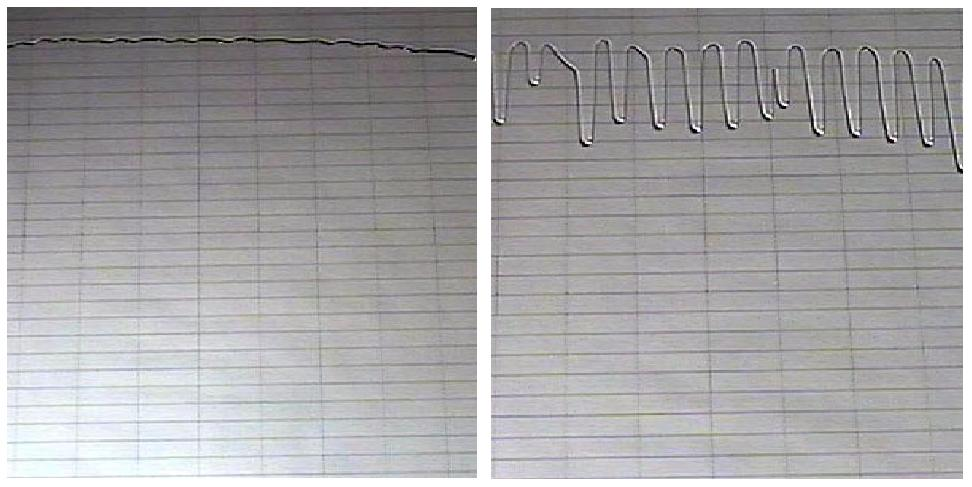
\includegraphics[width=.9\textwidth]{./Slike/film-slika}
\caption{Polzenje tanke plasti teko"cine po nagnjeni povr"sini. Majhne motnje v obliki fronte (levo) hitro prerastejo v vzorec, ki ni niti pribli"zno enakomeren, je pa periodi"cen (desno). Vir: \cite{kondic}}
\label{fig:film-neenakomernost}
\end{figure}

Vzorec na sliki~\ref{fig:film-neenakomernost} lahko pojasnimo s kratkim razmislekom. Po klan"cini navzdol vodo poganja sila te"ze, zadr"zujeta pa jo viskoznost in povr"sinska napetost, ki pa imata velik vpliv le na tanke plasti. "Ce majhna motnja ob nekem trenutku povzro"ci, da je na nekem mestu plast voda debelej"sa, imata tako viskoznost kot povr"sinska napetost manj"si vpliv na gibanje vode kot sila te"ze, zato bo na tistem mestu steklo ve"c vode kot drugod, kar bo le okrepilo za"cetno motnjo, tako da bo na tistem mestu voda vedno la"zje tekla. 

Le z razmislekom pa ne znamo napovedati niti kon"cne oblike fronte niti povpre"cne razdalje med mesti z ve"cjim pretokom. "Ce nas to zanima, moramo tudi kaj izra"cunati. 

\subsection{Ena"cbe}

"Ce privzamemo nestisljivost teko"cine $\nabla \cdot \vec u = 0$, se Navier-Stokesova ena"cba za teko"cino na klan"cu poenostavi v 

\begin{align}
 \label{eq:ns-film}
 \frac{\partial \vec u}{\partial t} + (\nabla \cdot \vec u) &= -\frac{1}{\rho}\nabla p + \frac{\mu}{\rho}\nabla^2 \vec u + g (\sin \alpha \vec i - \cos \alpha \vec k)
\end{align}

kjer je $\vec u$ hitrost teko"cine, $\rho$ njena gostota in $\mu$ viskoznost. "Clena z $g$ sta dinami"cna in stati"cna komponenta sile te"ze. Pomembni so tudi robni pogoji, obi"cajno se izbere slede"ce:

\begin{itemize}
 \item Na meji med teko"cino in klancem teko"cina ne drsi, torej je tam $\vec u = 0$. 
 \item Na meji med teko"cino in zrakom ima tlak nezveznost, ki jo sorazmerja povr"sinski napetosti in ukrivljenosti meje $\kappa$. 
\end{itemize}

Ker obravnavamo tanke filme, lahko privzamemo, da je debelina $h$ manj"sa od katerekoli dol"zinske skale v ravnini. S tem privzetkom lahko ena"cbo (\ref{eq:ns-film}) poenostavimo v ena"cbo za $h$. 

\begin{align}
\label{eq:ns-film-h}
 \frac{\partial h}{\partial t} = -\frac{1}{3\mu}\nabla \cdot \left[ \gamma h^3 \nabla \nabla^2 h - \rho g h^3 \nabla h \cos \alpha + \rho g h^2 \sin \alpha \vec i \right]
\end{align}

\begin{figure}[h]
\centering
 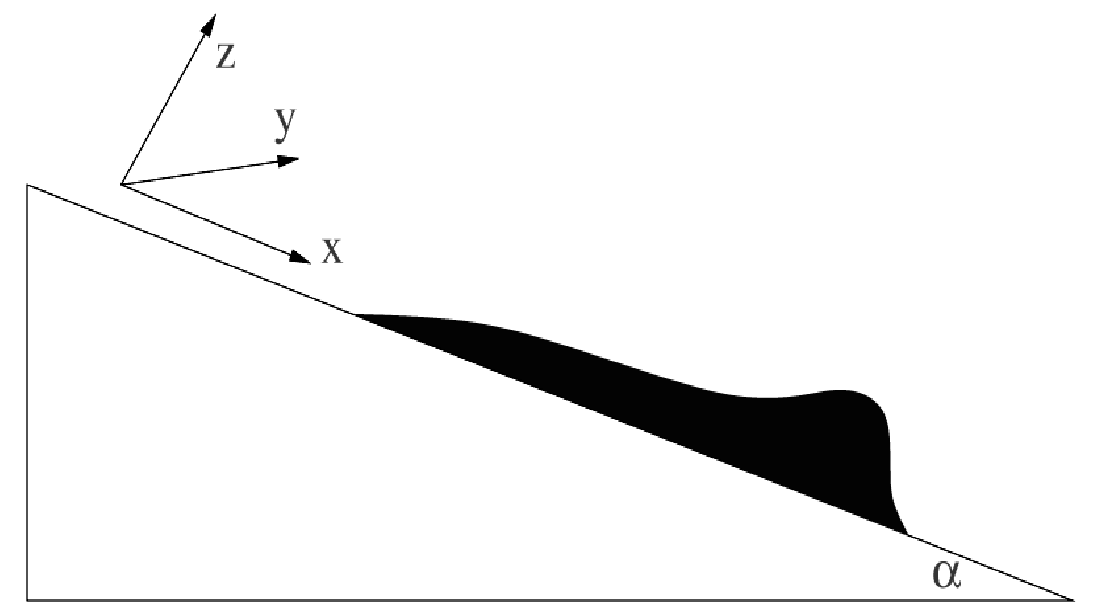
\includegraphics[width=.8\textwidth]{./Slike/film-skica}
\caption{Skica teko"cine v dveh dimenzijah. Viden je greben tik za fronto teko"cine in pa zo"zitev dale"c za fronto, ki je pri ra"cunih ne bomo upo"stevali}
\label{fig:film-skica}
\end{figure}

\subsection{Re"sevanje}

Zgornja ena"cba je "se vedno prezahtevna, da bi jo re"sevali analiti"cno, zato pose"zemo po numeri"cnih metodah. 

\subsection{Nestabilnost}

Osnovna re"sitev $h_0(x, t)$ je sicer odvisna od "casa, vendar lahko predpostavimo, da rob teko"cine polzi s konstantno hitrostjo $U$. "Casovno odvisnost koeficientov $h_0$ bomo torej odpravili, "ce se postavimo v koordinatni sistem, ki se giblje s to hitrostjo. V tem primeru uvedemo spremenljivko $\xi = x - Ut$ in $\nabla = (\partial_\xi, \partial_y)$, splo"sno re"sitev pa lahko zapi"semo v obliki

\begin{equation}
 h(\xi, y, t) = h_0(\xi) + \eps h_1(\xi, y, t)
\end{equation}

V tej sliki se $h_0$ ne spreminja s "casom, torej smo dobili linearno diferencialno ena"cbo s konstantnimi koeficienti. Ker "zelimo, da je motnja res majhna, predpostavimo, da sta $h_0$ in $h_1$ podobnega velikostnega reda, $\eps$ pa zelo majhen, dosti manj"si od 1. Zgornji izraz vstavimo v ena"cbo (\ref{eq:ns-film-h}) in zanemarimo vse "clene z drugi in vi"sjimi potencami $\eps$. 

Na sliki~\ref{fig:film-neenakomernost} vidimo, da je oblika fronte pribli"zno periodi"cna, zato $h_1(\xi, y, t)$ raje zapi"semo kot linearno kombinacijo normalnih valovnih na"cinov. V ena"cbi bo tako nastopala Fourierova transformiranka po koordinati $y$, ki jo ozna"cimo z $g(\xi, q, t)$, za katero velja

\begin{align}
 \odv{g} = -\mathcal{L}g
\end{align}

Tu je $\mathcal{L}$ linearni diferecialni operator s konstantimi koeficienti. Zanimajo nas lastne vrednosti tega operatorja, zlasti tista z najve"cjim realnim delom. Lastne vrednosti so odvisne od valovnega "stevila $q$ oz valovne dol"zine $\lambda = 2\pi/q$; pri"cakujemo, da bo valovna dol"zina, pri kateri je lastna vrednost $s(q)$ najve"cja, enaka razdalji med posameznimi pasovi na sliki~\ref{fig:film-neenakomernost}, saj bo motnja s tak"sno valovno dol"zino najhitreje nara"s"cala. 

Ker smo osnovno re"sitev $h_0$ izra"cunali numeri"cno, tudi matri"cne elemente operatorja $\mathcal{L}$ poznamo le numer"cno. 

\section{Podobni pojavi}

Polzenje teko"cine po klancu seveda ni edini hidrodinamski pojav, kjer lahko opazimo nestabilnosti. Ker je to zelo "siroko podro"cje, tu omenjam predvsem tak"sne pojave, ki so neposredno povezani s tokom tankih plasti teko"cin. 

\subsection{Milni mehur"cki}

\begin{figure}[h]
 \centering
\subfigure{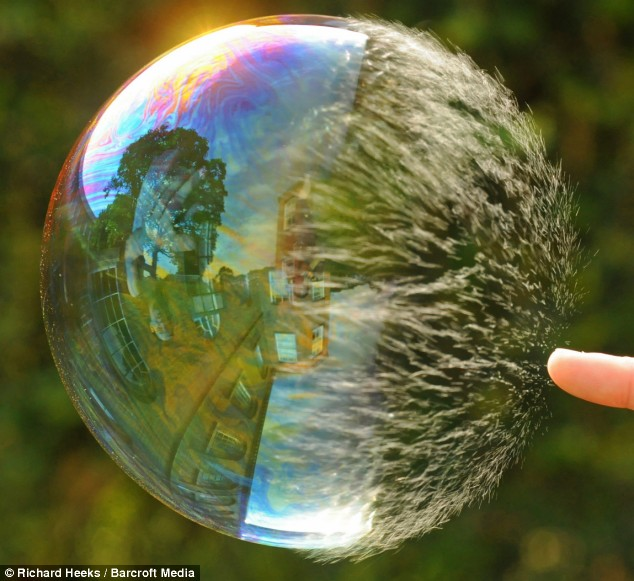
\includegraphics[height=.45\textwidth]{./Slike/bubble-3}}
\subfigure{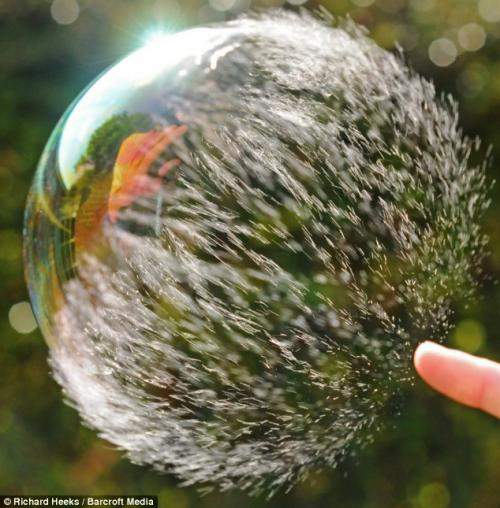
\includegraphics[height=.45\textwidth]{./Slike/bubble-4}}
\caption{Razpad milnega mehur"cka~\cite{slike-mehurcek}. }
\label{fig:mehurcek-3}
\end{figure}

Milni mehur"cki so stabilni na majhne motnje zaradi povr"sinske napetosti teko"cine. "Ce pa mehur"cek predremo v eni to"cki, ustvarimo rob, kjer povr"sinska napetost ni uravnote"zena, zato se rob za"cne umikati. Ker je opna obi"cajno zelo tanka, 
je ukrivljenost na robu velika, zato fronta napreduje zelo hitro~\cite{diploma}. To napredovanje je pri mehur"ckih tako hitro, da s prostim o"cesom fronte sploh ne opazimo, ampak se nam zdi, da celoten mehur"cek razpade naenkrat. 
 

Podobno kot pri tankem filmu tudi tu obravnavamo tanko plast teko"cine pod vplivom povr"sinske napetosti. Pojava pa se mo"cno razlikujeta pri viru nestabilnosti. Pri razpadu milnega mehur"cka namre"ce ne opazimo nestabilnosti v obliki fronte, ampak v dejstvu, da opna razpade v kapljice. 

\begin{comment}

lahko tudi za opno predpostavimo, da je tanka, njeno debelino pa ozna"cimo s $h = h(x,t)$. Opna ima translacijsko simetrijo v smeri $y$, zato na za"cetku predpostavimo, da imajo tak"sno simetrijo tudi $h$ ter gostota in tlak teko"cine. 

\begin{figure}
 \centering
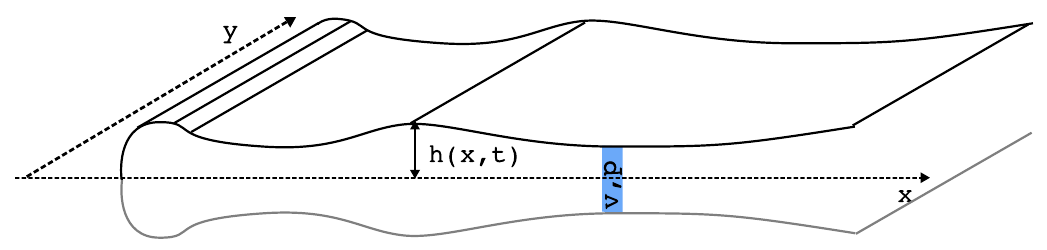
\includegraphics[width=.8\textwidth]{./Slike/mehurcek-skica}
\caption{Profil opne s translacijsko simetrijo vzdol"z roba in zrcalno simetrijo v navpi"cni smeri. Ker je opna tanka, lahko privzamemo, da se tlak in hitrost ne spreminjata po debelini~\cite{diploma}. }
\label{mehurcek-skica}
\end{figure}

\subsubsection{Gibalna ena"cba}

Tok neviskozne in nestisljive teko"cine opisuje Eulerjeva ena"cba

\begin{equation}
\label{eq:meh-euler}
 \odv{\vec v} + (\vec v \cdot \nabla)\vec v = - \nabla p
\end{equation}

Hkrati pa za opno velja tudi ohranitev prostornine, ki jo v brezdimenzijski obliki zapi"semo kot

\begin{equation}
\label{eq:meh-ohranitev}
 \odv{h} + \nabla (h\vec v) = 0
\end{equation}

\subsubsection{Ohranitev energije}
Vemo, da opna za fronto razpade v kapljice. Njihovo "stevilo in velikost lahko dolo"cimo iz ohraniev energije in skupne prostornine. Pred razpadom je edini prispevek k energiji povr"sinska napetost opne, po razpadu pa nastane $N$ enako velikih kapljic z radijem $r$ in hitrostjo $v$. Ohranitev energije ob razpadu odseka opne s povr"sino $S$ da enakost

\begin{equation}
 \sigma N 4 \pi r^2 + 2 S h_0 \rho \frac{v^2}{2} = 2S\sigma
\end{equation}

kjer je prvi "clen energija povr"sinske napetosti kapljic, drugi kineti"cna energija kapljic, na desni pa energija opne pred razpadom. Zvezo med povr"sino opne $S$ in "stevilom kapljic $N$ dobimo iz ohranitve volumna, tako da se ohranitev energije v brezdimenzijski obliki, kjer je $r$ v enotah $h_0$, $v$ pa v enotah $v_0 = \sqrt{\frac{\sigma}{\rho h_0}}$, glasi

\begin{equation}
 \frac{3}{r} + \frac{v^2}{2} = 1
\end{equation}

\subsubsection{Potujo"ci valovi}

Drugo zvezo med velikostjo in hitrostjo kapljic pa dobimo ob predpostavki, da fronta s "casom ohranja svojo obliko, torej jo lahko zapi"semo kot potujo"ci val. Ker se premika le v eni smeri, uporabimo valovno ena"cbo prvega reda

\begin{equation}
 \frac{\partial v}{\partial t} + c \nabla v = 0
\end{equation}

"Ce bi bila hitrost valovanja $c$ manj"sa od hitrosti teko"cine na robu $v$, bi bilo gibanje teko"cine nadzvo"cno in bi nastajali udarni valovi. "Ce pa bi bila motnja hitrej"sa od teko"cine, bi opna razpadala "ze pred fronto. Edina smiselna mo"znost je torej, da je $c=v$. 

\end{comment}

\subsection{Kra"ski "zlebi"ci}

% TODO: Citat, dobi diplomo od Kodreta

\begin{figure}[h]
\centering
 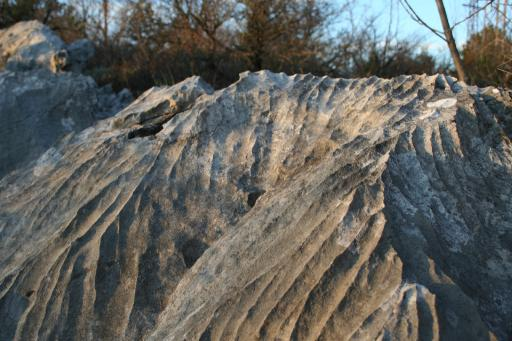
\includegraphics[width=.8\textwidth]{./Slike/Zlebici}
 \caption{"Zlebi"ci na slovenskem Krasu pri Nabre"zini~\cite{wiki:zlebic} }
 \label{fig:zlebici-slika}
\end{figure}

S slike~\ref{fig:zlebici-slika} lahko vidimo, da "zlebi"ci tvorijo podobno periodi"cno strukturo kot teko"cina na sliki~\ref{fig:film-neenakomernost}. Tudi po izvoru sta pojava sorodna: Na tistih mestih, kjer "cez "zlebi"c ste"ce ve"c vode, se tudi raztopi ve"c apnenca, torej postane kanal "se globlji in skozenj te"ce "se ve"c vode. 

Plast teko"cine tu seveda ni tako tanka, da bi povr"sinka nepotest igrala veliko vlogo, je pa "se vedno debelina toka $h$ dosti manj"sa od velikosti pobo"cja, na katerem se tvorijo "zlebi"ci. 


\subsection{Razpad curka}

Na nestabilnosti pogosto naletimo tudi pri "studiju razpada curkov teko"cin~\cite{eggers}. 

\section{Zaklju"cek}

\begin{thebibliography}{3}
  \bibitem{diploma} S. "Copar, Numeri"cna analiza nestabilnosti na robu teko"cinske opne, Diplomsko delo (2009)
  \bibitem{kondic} L. Kondic, SIAM Review \textbf{45}, 95 (2003)
  \bibitem{eggers} J. Eggers in E. Villermaux, Rep. Prog. Phys. \textbf{71}, 036601 (2008)
  \bibitem{drazin} P. G. Drazin, \textit{Introduction to hydrodynamic stability}, Cambridge University Press (2002)
  \bibitem{slike-mehurcek} \url{http://www.dailymail.co.uk/sciencetech/article-1199149/Super-slow-motion-pictures-soap-bubble-bursting-stunning-detail.html} (23. 1. 2012)
  \bibitem{wiki:zlebic} \href{http://sl.wikipedia.org/wiki/\%C5\%BDlebi\%C4\%8Di}{http://sl.wikipedia.org/wiki/\v Zlebič} (2. 2. 2012)
\end{thebibliography}


\end{document}
